\documentclass{article}


% if you need to pass options to natbib, use, e.g.:
%     \PassOptionsToPackage{numbers, compress}{natbib}
% before loading neurips_2022


% ready for submission
\usepackage{neurips_2022}


% to compile a preprint version, e.g., for submission to arXiv, add add the
% [preprint] option:
%     \usepackage[preprint]{neurips_2022}


% to compile a camera-ready version, add the [final] option, e.g.:
%     \usepackage[final]{neurips_2022}


% to avoid loading the natbib package, add option nonatbib:
%    \usepackage[nonatbib]{neurips_2022}


\usepackage[utf8]{inputenc} % allow utf-8 input
\usepackage[T1]{fontenc}    % use 8-bit T1 fonts
\usepackage{hyperref}       % hyperlinks
\usepackage{url}            % simple URL typesetting
\usepackage{booktabs}       % professional-quality tables
\usepackage{amsfonts}       % blackboard math symbols
\usepackage{nicefrac}       % compact symbols for 1/2, etc.
\usepackage{microtype}      % microtypography
\usepackage{xcolor}         % colors

\usepackage{amsmath}
\usepackage{amsfonts}
\usepackage{amssymb}
\usepackage{graphicx}
\usepackage{algorithm}
\usepackage{algpseudocode}
\usepackage{blindtext}
\usepackage{hyperref}
\usepackage{amsthm}
\usepackage{subfig}
\usepackage{textcomp}
\usepackage{comment}

\newcommand{\cov}{\mathrm{cov}}
\newcommand{\corr}{\mathrm{corr}}
\newcommand{\var}{\mathrm{var}}
\newcommand{\CE}{\mathrm{CE}}
\newcommand{\KacIM}{\mathrm{KacIM}}

%\usepackage{prletters}

\newtheorem{theorem}{Theorem}
\newtheorem{collorary}{Collorary}

\title{Measuring statistical dependencies via maximum norm and characteristic functions}


% The \author macro works with any number of authors. There are two commands
% used to separate the names and addresses of multiple authors: \And and \AND.
%
% Using \And between authors leaves it to LaTeX to determine where to break the
% lines. Using \AND forces a line break at that point. So, if LaTeX puts 3 of 4
% authors names on the first line, and the last on the second line, try using
% \AND instead of \And before the third author name.


\author{%
  David S.~Hippocampus\thanks{Use footnote for providing further information
    about author (webpage, alternative address)---\emph{not} for acknowledging
    funding agencies.} \\
  Department of Computer Science\\
  Cranberry-Lemon University\\
  Pittsburgh, PA 15213 \\
  \texttt{hippo@cs.cranberry-lemon.edu} \\
  % examples of more authors
  % \And
  % Coauthor \\
  % Affiliation \\
  % Address \\
  % \texttt{email} \\
  % \AND
  % Coauthor \\
  % Affiliation \\
  % Address \\
  % \texttt{email} \\
  % \And
  % Coauthor \\
  % Affiliation \\
  % Address \\
  % \texttt{email} \\
  % \And
  % Coauthor \\
  % Affiliation \\
  % Address \\
  % \texttt{email} \\
}


\begin{document}


\maketitle


\begin{abstract}
    In this paper we focus on the problem of statistical dependence estimation. We propose statistical dependence measure based on the maximum-norm of the absolute value of difference between joint and product-marginal characteristic functions, and its iterative estimation algorithm. The proposed measure is differentiable, can be efficiently applied to high-dimensional data, and integrated into modern machine learning pipelines. We also conduct experiments both with simulated and real data, which reveal that the proposed measure can exploit statistical dependence in non-linear data sets more efficiently, comparing to the previous work in this line of research, and that it can improve real-data classification accuracy, when applied for feature extraction and regularisation.
\end{abstract}

\section{Introduction}
The measurement of  statistical dependence plays important role in various empirical learning methods (e.g. hypothesis testing~\cite{Gretton2005MeasuringSD}, feature selection and extraction~\cite{EigenHSIC,HSCA}, information bottleneck methods \cite{Ma2020TheHB}, causal inference~\cite{NIPS2008_f7664060}, self-supervised learning~\cite{li2021selfsupervised}, representation learning~\cite{Ragonesi2021LearningUR}, among others).  Hystorically, earliest statistical dependence estimation ideas (e.g. conditional probability) share nearly-common origin with the beginning of formal statistical reasoning itself. During last two centuries ideas of correlation and (relative) entropy (including various generalizations) were proposed and became very popular in numerous applications and theoretical developments. However, with the increasing growth of machine and deep learning, new statistical dependence estimation methods, that are robust, applicable to noisy, high-dimensional, structured data, and which can be efficiently integrated with modern machine learning and deep learning methods are helpful for the development both of the theory and application.

In this article we focus on quantitative estimation of statistical depdendencies, using characteristic functions. We begin with the short review of some important previous dependence estimation approaches (Section~\ref{section:previous_work}), devoting special attention to ones based on characteristic functions (Section~\ref{section:previous_work_cf}). Afterwards, in (Section~\ref{section:proposed_method}), we formulate the proposed measure, its empirical estimator, and conduct preliminary theoretical analysis, which are the main theoretical contribution of our paper. Section~\ref{section:experiments} is devoted to experiments with simulated and real data sets, where we apply the proposed statistical measure for feature extraction and deep neural network (DNN) regularisation. Finalizing Section~\ref{section:conclusion} discusses and concludes this article.


\section{Previous Work}
\label{section:previous_work}
During recent years, various approaches have been used in order to construct statistical dependence estimation methods. For example, information theory (mutual information ~\cite{Cover2006} and generalisations), reproducing kernel Hilbert spaces (Hilbert-Schmidt independence criterion \cite{Gretton2005MeasuringSD}), characteristic functions (distance correlation~\cite{Feuerverger, Szekely}), and other (e.g. ~\cite{Pczos2012CopulabasedKD} copula-based kernel dependence measures, integral-porbability-metric-reliant Sobolev independence criterion~\cite{NIPS2019_9147}).
Further we will focus on characteristic-function-based methods. 

\subsection{Characteristic-function-based methods}
\label{section:previous_work_cf}
Characteristic function (CF) of $d_{X}$-dimensional random vector $X$ defined in some probability space $(\Omega_{X}, \mathcal{F}_{X}, \mathbb{P}_{X})$ is defined as: 
\begin{equation}
\label{eq:characteristic_function}
\phi_{X}(\alpha): = \mathbb{E}_{X} e^{i\alpha^{T}X}, 
\end{equation}
where $i=\sqrt{-1}$, $\alpha \in R^{d_{X}}$. Having $n$ i.i.d. realisations of $X$, corresponding empirical characteristic function (ECF) is defined as:
\begin{equation}
\label{eq:ecf}
\widehat{\phi_{X}}(\alpha): = \frac{1}{n} \sum_{j=1}^{n} e^{i <\alpha, x_{j}>}.
\end{equation}
Having pair of two random vectors $(X,Y)$ defined in another probability space $(\Omega_{X,Y}, \mathcal{F}_{X,Y}, \mathbb{P}_{X,Y})$  joint CF is defined as:
\begin{equation}
\label{eq:joint_characteristic_function}
\phi_{X,Y}(\alpha,\beta): = \mathbb{E}_{X,Y} e^{i(\alpha^{T}X + \beta^{T}Y)},
\end{equation}
where $\alpha \in \mathbb{R}^{d_{X}}$ and $\beta \in \mathbb{R}^{d_{Y}}$. Similarly, having 
$n$ i.i.d. realisations of $(X,Y)$, joint ECF is defined as:
\begin{equation}
\label{eq:joint_ecf}
\widehat{\phi_{X,Y}}(\alpha,\beta): = \frac{1}{n} \sum_{j=1}^{n} e^{i(<\alpha, x_{j}> + <\beta, y_{j}>) }.
\end{equation}


Uniqueness theorem states that two random variables $X$ and $Y$ have the same distribution if and only if their CF's are identical \cite{?}. Therefore, CF's can be regarded as an alternative description of distribution. Roughly speaking, CF can be regarded as Fourier transform of probability density funciton (PDF).

If cumulative distribution function (CDF) of $(X,Y)$, $F_{X,Y}(x,y)$, $x \in \mathbb{R}^{d_{X}}$ and $y \in \mathbb{R}^{d_{Y}}$ factorises as $F_{X}(x)F_{Y}(y)$ for all $x$ and $y$, $X$ and $Y$ are called independent (the same holds for probability density function, PDF). However, this criterion is impractical due to need of evaluation of potentially high-dimensional CDF or PDF, and often alternative independence criterions are more useful. Let us define 

\begin{equation}
%\mathbb{E}_{X,Y} e^{i <\alpha, X> + i <\beta, Y>} = \mathbb{E}_{X} e^{i <\alpha, X>} \mathbb{E}_{Y} e^{i <\beta, Y>},
\label{eq:kac_theorem}
\Delta_{X,Y}(\alpha, \beta) := \phi_{X,Y}(\alpha,\beta) - \phi_{X}(\alpha) \phi_{Y}(\beta),
\end{equation}
%where $d_{x}$ and $d_{y}$ are dimensions of $X$ and $Y$, respectively.
an its empirical counterpart:
\begin{equation}
\label{eq:empirical_delta}
\widehat{\Delta}_{X,Y}(\alpha, \beta) := \widehat{\phi}_{X,Y}(\alpha,\beta) - \widehat{\phi}_{X}(\alpha) \widehat{\phi_{Y}}(\beta).
\end{equation}

In terms of CF's, statistical independence  of $X$ and $Y$ is equivalent to $\forall \alpha \in \mathbb{R}^{d_X},\forall \beta \in \mathbb{R}^{d_Y} $, $\Delta_{X,Y}(\alpha, \beta) = 0$~\cite{KacTheorem}.

Historically, $\Delta_{X,Y}(\alpha, \beta)$ was used as the basis (first in~\cite{Feuerverger} for one-dimensional case, and afterwards extended and developed by~\cite{Szekely} for bivariate multidimensional random vectors) for construction of statistical independence tests and measures. Distance covariance and distance correlation, prosposed by ~\cite{Szekely} relies on weighted $L^{2}$-norm analysis of~\eqref{eq:kac_theorem}. They select weighting function in such a way, that dependence measure can be expressed in terms of correlection of data-dependent distances. Recent result of~\cite{Bottcher} generalises~\cite{Szekely} to multivariable case.~\cite{CHAUDHURI201915} proposed computationally efficient algorithm for estimation of distance correlation measure, reducing computational complexity from $O(n^2)$ to $O(n\cdot \log n)$, where $n$ is sample size.

\textbf{Motivation and Connection To Previous Work} 
Taking $\Delta_{X,Y}(\alpha, \beta) = 0$~\eqref{eq:kac_theorem} as the criterion of statistical independence we view the work~\cite{Szekely} from the perspective of weighted $L^{p}$ spaces, measuing statistical dependence by the corresponding $L^{p}$-norms of~\eqref{eq:kac_theorem}.

Taking into account that~\cite{Szekely} in high dimensions is affected with the curse of dimensionality~\cite{Edlemann}, we focus on the limit case $p \rightarrow \infty$($L^{\infty}$ space), which is associated to the supremum norm. This norm has several potential advantages.



We hypothesise, that its locality could be exploited to detect statistical independence more efficiently, comparing to case $p=2$. 
In addition, numerically calculation of $L^{\infty} $ norm would not require to directly calculate norm integral, since norm of $L^{p}$ converges to supremum norm when $p \rightarrow \infty$. Also, from practical point of view maximization is convenient, because it is efficiently implemented in modern deep learning frameworks (e.g. Pytorch~\cite{NEURIPS2019_9015}). 
In addition, in our opinion it is worth to note, that applications of characteristic functions in machine learning are quite scarce, despite that they provide quite convenient theoretical proxy to access distributions.

\section{Proposed Measure}
\label{section:proposed_method}
% sparse vectors - PAC style theorem ?



\noindent The above considerations serves as the basis for constructing of a novel dependence measure, which we further refer to as Kac independence measure (KacIM). Having two random vectors $X$ and $Y$, KacIM is defined as
\begin{equation}
\label{eq:kim}
\kappa(X,Y):= \max_{\alpha \in \mathbb{R}^{d_{X}}, \beta \in \mathbb{R}^{d_{Y}}} |\Delta_{X,Y}(\alpha,\beta)|.
\end{equation}

%In contrary to~\cite{Szekely} the proposed~\eqref{eq:kim} measure relies on maximum norm of difference between joint and product-marginal characteristic functions.

\subsection{Basic Properties}
\begin{theorem}
	\label{thm:properties}
	KacIM~\eqref{eq:kim} has the following properties:
	\begin{enumerate} 
		\item $\kappa(X,Y) = \kappa(Y,X)$,
		\item $0 \leq \kappa(X,Y) \leq 1$,
		\item $\kappa(X,Y) = 0$ iff $X\perp Y$.
	\end{enumerate}    
\end{theorem}


\begin{proof}
	Property $\textit{1.}$ is obvious from definition~\eqref{eq:kim} (commutativity of addition and multiplication), and property $\textit{2.}$ directly follows from Cauchy inequality and that absolute value of CF is bounded by $1$:
	\begin{multline*}
	|\phi_{X,Y}(\alpha, \beta)  -\phi_{X}(\alpha) \phi_{Y}(\beta)|^{2} =
	\mathbb{E}_{X,Y} |( e^{i\alpha^{T}X} - \phi_{X}(\alpha) )(e^{i\beta^{T}Y}- \phi_{Y}(\beta) )|^{2} \leq \\
	\mathbb{E}_{X,Y} |( e^{i\alpha^{T}X} - \phi_{X}(\alpha) )|^{2} |(e^{i\beta^{T}Y}- \phi_{Y}(\beta) )|^{2}  = (1 - |\phi_{X}(\alpha)|^{2}) (1 - |\phi_{Y}(\beta)|^{2}).
	\end{multline*}
	Proof of property $\textit{3.}$ directly follows from properties of CF's (see e.g.~\cite{Jacod}, Corollary 14.1)\footnote{This property also is known as Kac's theorem~\cite{KacTheorem}. Although it is quite simple mathematical fact, this provides the basis of the proposed measure's name.}.	
\end{proof}

Although~\eqref{eq:kim} is not scale invariant in general, scale invariance can be achieved by assuming standartization of $X$ and $Y$.


\subsection{Estimation}

Having i.i.d. observations $(x_{j}, y_{j})$, $j = 1,2,...,n$, an empirical estimator of~\eqref{eq:kim} is defined via corresponding ECF's~\eqref{eq:joint_ecf} and~\eqref{eq:ecf}:
\begin{equation}
\label{eq:estimator}
\hat{\kappa}(X,Y) := \max_{\alpha, \beta} \vert \widehat{\Delta}_{X,Y}(\alpha, \beta) \vert =\max_{\alpha, \beta} \vert \widehat{\phi_{X,Y}}(\alpha,\beta)  - \widehat{\phi_{X}}(\alpha) \widehat{\phi_{Y}}(\beta) \vert.
\end{equation}

\noindent By \textit{Levy continuity theorem} \cite{LCT} ECF converges to CF. Therefore empirical estimator~\eqref{eq:estimator} converges (?) into KacIM~\eqref{eq:kim} (in what sense, check?).

\noindent It can be calculated iteratively by Algorithm~\ref{alg:estimator_computation} (Pytorch~\cite{NEURIPS2019_9015} implementation can be accessed from \url{https://github.com/povidanius/kac_independence_measure}). 


\begin{algorithm}
	\caption{KacIM estimation}\label{alg:estimator_computation}
	\begin{algorithmic}
		\Require Number of iterations $N$, gradient-based optimiser $GradOpt([parameters],.)$, initial $\alpha \in \mathbb{R}^{d_{X}}, \beta \in \mathbb{R}^{d_{Y}}$.
		\For{iteration=1 to N}
		\State Sample data batch $(X,Y):=(x_{i},y_{i})_{i=1}^{n_{b}}$.
		\State Normalize $(X,Y)$ to zero mean and unit variance (scale invariance).
		\State Calculate  $\widehat{\Delta}_{\alpha, \beta}(X,Y)$.
		\State Perform one maximization iteration of $\widehat{\Delta}(X,Y)$ via $\alpha, \beta \rightarrow GradOpt([\alpha, \beta], \widehat{\Delta}_{\alpha, \beta}(X,Y))$.
		\EndFor
	\end{algorithmic}
\end{algorithm}



Algorithm~\ref{alg:estimator_computation} requires to initialise $\alpha$ and $\beta$, and optimiser. In our implementation we use uniform initialisation of parameters, and decoupled weight decay regularization optimizer~\cite{Loshchilov2019DecoupledWD}. 
We also empirically observed that normalisation of parameters $\alpha$ and $\beta$ on to unit sphere increases estimation stability. After the estimation of KacIM via Algorithm~\ref{alg:estimator_computation}, the evaluation the estimator  has computation complexity $O(n)$, where $n$ is sample size.

Note, that mutual information~\cite{Cover2006} (and $f$-divergence-based analogues in general) are also estimated via transforming them into maximisation problem by Donsker-Varadhan representation~\cite{pmlr-v80-belghazi18a}, in order to avoid density estimation. In this case, optimisation is conducted over the space of neural network parameters, which is substantially larger than the number of parameters needed to estimate $KacIM$ (i.e. $d_{x} + d_{y}$ parameters).

\subsection{Interpretation and connection previous approaches}
\textbf{Interpretation in general case}. Since \eqref{eq:kim} can be reformulated as
\begin{equation}
\kappa(X,Y) = \max_{\alpha,\beta} |\cov(e^{i\alpha^{T}X},e^{i\beta^{T}Y})|,
\end{equation}
by Euler's formula, it corresponds to the maximum pseudocovariance between complex exponents $e^{i\alpha^{T}X} = cos(\alpha^{T}X) + i \cdot sin(\alpha^{T}X)$ and $e^{i\beta^{T}Y} = cos(\beta^{T}Y) + i \cdot sin(\beta^{T}Y)$.
Since $\var(e^{i\alpha^{T}X}) = \phi(2\alpha) - \phi(\alpha)^2$, one can also define the normalised version of KacIM (refine or remove this):
%\begin{comment}
\begin{equation}
\kappa_{norm}(X,Y) = \max_{\alpha,\beta} |\corr(e^{i\alpha^{T}X},e^{i\beta^{T}Y})| = \max_{\alpha,\beta}  \frac{|\cov(e^{i\alpha^{T}X},e^{i\beta^{T}Y})|}{\sqrt{|\phi_{X}(2\alpha)-\phi_{X}^{2}(\alpha)||\phi_{Y}(2\beta)-\phi_{Y}^{2}(\beta)|}}.
\end{equation}

%\end{comment}

\textbf{Interpretation in Gaussian case}. In special case when both $X$ and $Y$ are zero mean Gaussian random vectors we have:
\begin{equation}
\label{eq:gaussian_kacim}
\kappa(X,Y) = \max_{\alpha, \beta} | e^{-\frac{1}{2} (\alpha^{T}\Sigma_{x}\alpha + \beta{^T}\Sigma_{y}\beta)}(e^{-\alpha{^T}\Sigma_{x,y}\beta} - 1)|.
\end{equation}
Assuming constant $\alpha^{T}\Sigma_{x}\alpha$ and  $\beta{^T}\Sigma_{y}\beta$, the maximization corresponds to the maximization of  $\alpha{^T}\Sigma_{x,y}\beta$, which coincides with canonical correlation analysis~\cite{10.5555/3279302}. Here $\Sigma_{x}$, $\Sigma_{y}$, and  $\Sigma_{x,y}$ are covariance matrices of $X$, $Y$, and cross-covariance matrix between $X$ and $Y$, respectively.

%\textbf{Generative models}. In the environment of generative models  with Gaussian outputs (e.g. variational autoencoder), estimation of KacIM in equivalent to finding first cannonical correlation pair between corresponding outputs.



\section{Experiments}
\label{section:experiments}

Further we will conduct empirical investigation of KacIM in order to demonstrate that it can measure non-linear statistical dependencies, and that it can be practically useful as a component of cost functions (we investigate feature extraction, and regularisation problems).

\subsection{Generated data}

\paragraph{Non-linear statistical dependence detection.} We begin with simulated multivariate data with additive and multiplicative noise.


\begin{figure}%
	\centering
	\subfloat{{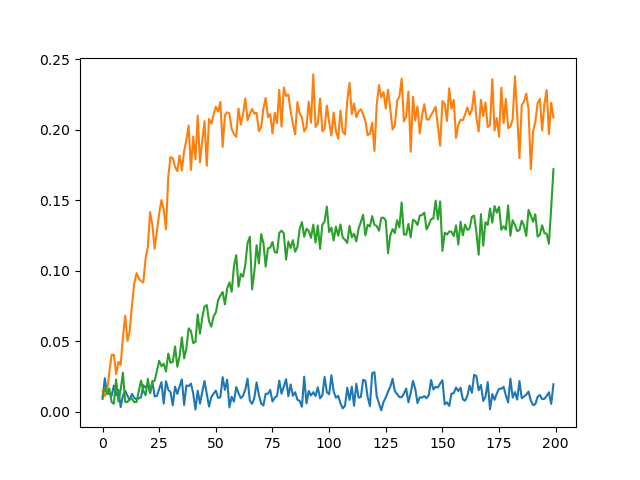
\includegraphics[scale=0.40]{../experiments/basic_demonstration/dependence_detection.png} }}%
	\qquad
	\subfloat{{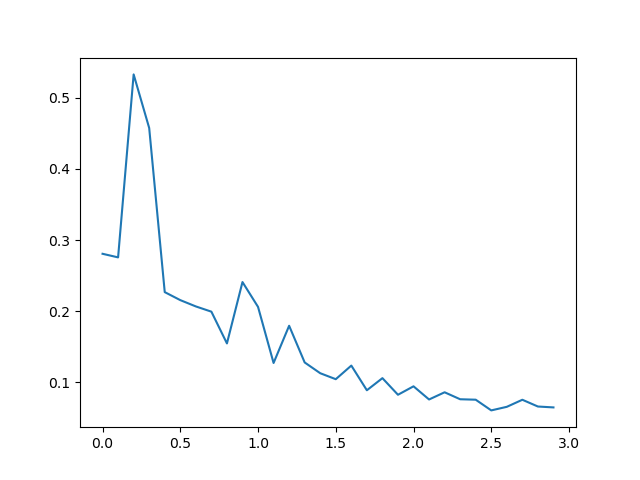
\includegraphics[scale=0.40]{../experiments/noise_effect/summary.png} }}%
	\caption{Left figure: KacIM evaluation for independent data (blue), additive (orange) and multiplicative (green) noise scenarios ($x$ axis - iteration, and $y$ - corresponding value of KacIM). Right figure: noise level ($x$ axis) vs final iteration KacIM value ($y$ axis). KacIM values for larger noise levels saturates as in tail of graph}
	\label{fig:experiments_simulation}
\end{figure}

Figure~\ref{fig:experiments_simulation} reflects KacIM values during iterative adaptation ($200$ iterations). In the case of independent data, both $x_{i}$ and $y_{i}$ ($d_{x} = 512$, $d_{y} = 4$) are sampled from gaussian distribution, independently. In the case of dependent data, an additive noise and multiplicative noise, the dependent variable is generated according to $y_{i} = sin(P x_{i}) + cos(P x_{i}) + \lambda \epsilon_{i}$ ($\lambda = 1.00$) and $y_{i} = (sin(P x_{i}) + cos(P x_{i})) \epsilon_{i}$, respectively, where $P$ is $d_{x} \times d_{y}$ random projection matrix, $\epsilon_{i} \sim N(0,1)$ and $\epsilon_{i} \perp x_{i}$.

When data is independent, both in additive and multiplicative cases, due to independence, estimator~\eqref{eq:estimator} is resistant to maximisation, and oscillates near zero. On the other hand, when the data is not independent, the condition~\eqref{eq:kac_theorem} is violated and maximization of estimator~\eqref{eq:estimator} is possible.
\paragraph{Noise variance effect} In this simulation we use the same additive noise setting as in previous paragraph, but evaluate all noise levels $\lambda \in [0.1, 3.0]$, with step $0.1$.
Figure~\ref{fig:experiments_simulation} empirically shows that value of KacIM  negatively correlates with noise level, and therefore the proposed measure is able not only to detect whether independence is present, but also to quantitatively evaluate it.

%Since in~\ref{alg:estimator_computation} we standartize data, KacIM is also scale-invariant (i.e. $\kappa(rx, ry) = \kappa(x,y)$), where $r>0$ is scale parameter.

\paragraph{Comparison with distance correlation} We also evaluated distance correlation~\cite{Szekely} on the same generated samples of data, comparing it with KacIM. From Figure.~\ref{fig:experiments_simulation_dcor} we see that as data dimensionality grows, for independent data, the values of measure not only is significantly larger than zero, but it also grows like values of measure of dependent data. This empirically demonstrates that distance correlation is affected by the curse of dimensionality. On the other side, KacIM even for larger dimensions oscilates near zero for independent data, and significantly deviates from zero for dependent data case, as indicated in right component of Figure.~\ref{fig:experiments_simulation_dcor}. 


\begin{figure}%
	\centering
	\subfloat{{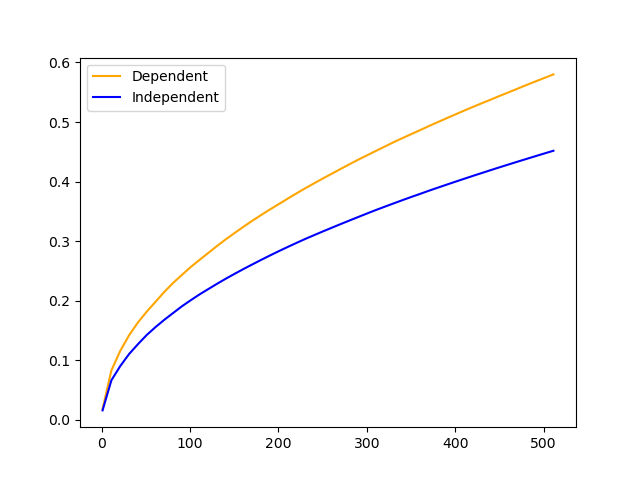
\includegraphics[scale=0.40]{../experiments/basic_demonstration/dependence_detection_dcor_dim.png} }}%
	\qquad
	\subfloat{{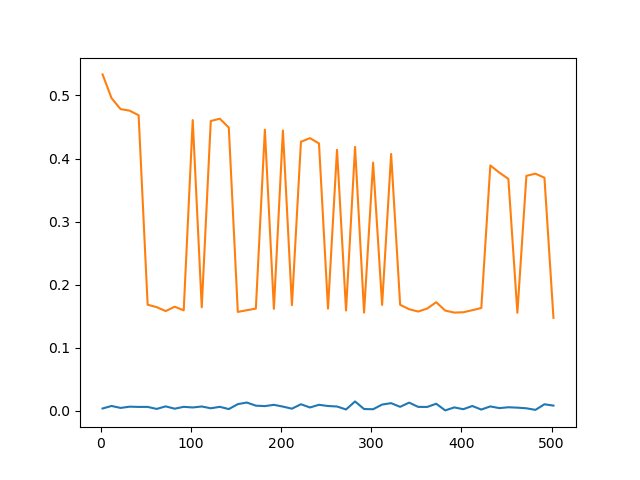
\includegraphics[scale=0.40]{../experiments/basic_demonstration/aaa_dependence_detection_kacim_by_dim_502.png} }}%
	
	\caption{The dimension of data is on the $x$ axis, and on $y$ axis is evaluation of distance correlation (left) and KacIM (right). Blue graph corresponds of independent data of dimension, indicated by $x$ axis, and orange one corresponds to dependent data.}
	\label{fig:experiments_simulation_dcor}
\end{figure}



\subsection{Feature extraction}

Previous work in the field of supervised feature extraction, which rely on dependency-based cost functions, include \cite{EigenHSIC,HSCA,10.1145/1839490.1839495} (HSIC),....().
%Further we will extend [?,?] algorithms in the dimension of the dependence measure, as the parameter. In our reasoining, and formulations we will adopt Bayesian framework, embodied in this probability factorisation:
%P(S|A,S') = F()/



Let use denote by $T := (x_{i},y_{i})_{i=1}^{N}$ a supervised-learning dataset of $N$ pairs of $d_{x}$-dimensional inputs $x_{i}$, and $d_{y}$-dimensional one-hot-encoded outputs $y_{i}$.

In feature extraction experiments we will use a set of classification data sets from OpenML~\cite{OpenML2013}, which cover different domains.  We use $KacIM$ in order to conduct supervised linear feature extraction by seeking 

\begin{equation}
\label{eq:kim_feature_extraction}    
W^{*} = arg \max_{W} \kappa(Wx, y) - \alpha Tr\{(W^{T}W-I)^{T}(W^{T}W-I) \},
\end{equation}
where the regularisation term, controlled by multiplier $\alpha \geq 0$, enforces semi-orthogonality of projection matrix $W^{*}$, and $Tr\{.\}$ denotes matrix trace operator.


In all the experiments~\eqref{eq:kim_feature_extraction} the cost function is optimised iteratively ($250$ iterations), simultaneously optimising parameters of KacIM ($\alpha$ and $\beta$) and projection matrix $W$.
After the optimisation, the feature extraction is conducted by $f(x) = W^{*}x$, where $x$ is original input vector, and $f$ are corresponding feature vector. 



We randomly split all the datasets in training and testing sets of equal size. % comparing unmodified inputs $x$, and features % of all possible dimensions up to $d_{x}$ with $10\%$ step.  
In our experiments we set $\alpha$ to $1.0$ to quickly ensure orthogonal projection matrices, and further proceed to dependence maximization stage. In order to quantitatively evaluate features, we use logistic regression classifier accuracy, measured on the testing set.


We use two baselines: raw features (RAW column in Table~\ref{table:classification_accuracies}) and neighborhood component analysis~\cite{NIPS2004_42fe8808} (NCA column in Table~\ref{table:classification_accuracies}).  The purpose of these experiments is to provide the preliminary evaluation of the applicability of KacIM for feature extraction, hence we use rather basic cost function and comparative baselines.




The classification accuracies, reported in Table~\ref{table:classification_accuracies} demonstrate that KacIM-based feature extraction procedure (KacIMFE column) indeed allows to increase classification accuracy when applied to real data sets from different domains, including high-dimensional and ill-defined ones (e.g. \textit{micro-mass} dataset). In contrast to our feature extraction approach, NCA explicitly optimises for classification accuracy, rather than more abstract dependency of features $f(x)$ with the dependent variable $y$.



\begin{table}	
	\centering
	\begin{tabular}{ |p{3cm}|p{2.0cm}|p{1.2cm}|p{1.7cm}|p{1.2cm}|  }
		%\hline
		%\multicolumn{5}{|c|}{Classification accuracies} \\
		\hline
		Dataset & $N$/$d_{x}$/$n_{c}$. & Raw & KacIMFE & NCA  \\
		\hline
		isolet & (7797,617,26)   &  0.9261  &  0.9437  &  \textbf{0.9477} \\
		madelon & (2600,500,2)   &  \textbf{0.6015}  &  0.5484  &  0.5685 \\
		prnn-viruses & (61,18,4)   &  0.6452  &  0.9265  &  0.9355 \\
		ionosphere & (351,34,2)   &  0.8807  &  0.9278  &  \textbf{0.9375} \\
		micro-mass & (360,1300,10)   &  0.8778  &  \textbf{0.9282}  &  0.8944 \\
		%CostaMadre1 & (296,37,2)   &  \textbf{0.8716}  &  0.8549  &  0.8378 \\
		clean1 & (476,168,2)   &  0.7689  &  \textbf{0.9888}  &  0.9790 \\
		%pc4 & (1458,37,2)   &  \textbf{0.8779}  &  0.8707  &  0.8683 \\
		robot-failures-lp2 & (47,90,5)   &  0.4583  &  0.6067  &  0.5833 \\
		waveform-5000 & (5000,40,3)   &  \textbf{0.8692}  &  0.8017  &  0.8516 \\
		spambase & (4601,57,2)   &  0.6906  &  0.8285  &  \textbf{0.8705} \\
		gina-agnostic & (3468,970,2)   &  \textbf{0.8512}  &  0.7894  &  0.8080 \\
		scene & (2407,299,2)   &  0.8895  &  \textbf{0.9707}  &  0.9336 \\
		tokyo1 & (959,44,2)   &  0.7250  &  0.8995  &  \textbf{0.9062} \\
		one-hundred-plants-shape & (1600,64,100)   &  0.1013  &  \textbf{0.4913}  &  0.4688 \\		
		
		\hline
	\end{tabular}
	\caption{Classification accuracies. $N$ denotes full data set size, $d_{x}$ - input dimensionality, and $n_{c}$ - number of classes. In this table feature dimension is equal to a half of original input dimension. Best accuracies that are also statistically significant (Wilcoxon's signed rank test~\cite{Wilcoxon1992}, 25 runs, $p$-value threshold $0.01$) are indicated in bold text.}
	\label{table:classification_accuracies}	
\end{table}




\subsection{Regularisation}
In regularisation experiments we investigate skin lession classification task. It is a binary classification data set, consisting of $10605$ images, which should be classified as benign or maligant (e.g. Figure~\ref{fig:Pneumonia_dataset_examples}).

We use \verb|ResNet18| backbone model (pretrained on ImageNet) with added classification head. Further we train this model with batches of $128$ elements.
We denote our classification network as $f(\phi(x|\theta_{0})|\theta_{1})$, where $\theta_{0}$ are parameters of \verb|ResNet18|, $\theta_{1}$ are classification head parameters, and $x$ is $224\times 224$ input image.
For optimisation we use decoupled weight decay regularization optimizer~\cite{Loshchilov2019DecoupledWD} with learning rate set to $0.0002$, and weight decay parameter set to $0.00001$ ($3$ epochs).
The internal learning rate of estimator (see\~ref{algo}) was set to $0.07$ and weight decay parameters to $0.01$.

\begin{figure}%
	\centering
	\subfloat{{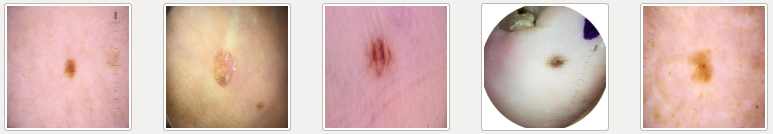
\includegraphics[scale=0.4]{./benign.png} }}%
	\qquad
	\subfloat{{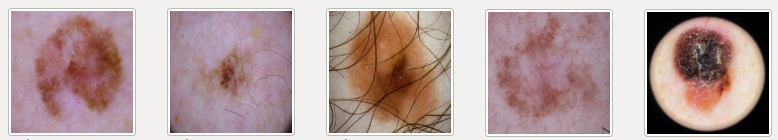
\includegraphics[scale=0.4]{./maligant.png} }}%
	\caption{Top figure - benign moles, bottom figure - maligant tumors.}
	\label{fig:Pneumonia_dataset_examples}
\end{figure}


We will investigate additive regularizer, which maximises depency of bottleneck the feature $\phi(x|\theta_{0})$ and target variable $y$ (one-hot encoding): 


\begin{equation}
\label{eq:regularizer1}
Cost(\theta_{0},\theta_{1}, W) := (1-\rho)\CE(f(\phi(x|\theta_{0})|\theta_{1}),y) - \rho \kappa(\phi(x|\theta_{0}),y),
\end{equation}

\noindent where $\CE(.,.)$ is cross-entropy loss, $\rho \geq 0$ is regularisation parameter (in our experiments $\rho = 0.2$). During backward pass, this regularizer is designed to directly transfer information from $y$ to the output \verb|ResNet18| $\phi(.|\theta_{0})$, and we hypothethise that this could provide possibility to learn more discriminative features.

\begin{table}	
	\centering
	\begin{tabular}{ |p{4cm}|p{3cm}|}
		%\hline
		%\multicolumn{5}{|c|}{Classification accuracies} \\
		\hline
		Mode & Average accuracy (\%)  \\
		\hline
		Without regularisation   &   93.01 \\		
		\hline
		With regularisation  &   \textbf{93.34} \\		
		\hline
	\end{tabular}
	\caption{Melanoma classification accuracy comparison of regularised and not regularised model. Bold text indicates that model with regulariser was more accurate (Wilcoxon's signed rank test~\cite{Wilcoxon1992}, 30 runs, $p$-value threshold $0.04$))}
	\label{table:regularisation_classification_accuracies}	
\end{table}


In each experiment we train classifier $30$ times with randomly splitted training and testing data ($9000$ images for training, and $1605$ for testing). The average accuracies reported in Table~\ref{table:regularisation_classification_accuracies}, that application~\eqref{eq:regularizer1} slightly (but with statistical significance) increased classification accuracy.

\section{Conclusion} 

\label{section:conclusion}
In this article we propose statistical dependence measure, KacIM, which corresponds to the $L^{\infty}$ norm of the absolute value of difference between joint characteristic function and the product of marginal ones. The proposed measure, in theory can detect non-linear statistical depdendence between a pairs of random variables of possibly different dimension, extended to various directions (e.g. kernels, multiple variables), applied to several machine learning tasks (e.g. feature extraction, regularisation, among others). On the other side, it raises a corresponding set of unanswered questions, both theoretical and empirical. 

For example, although it converges, the variance of the estimator sometimes is high and it is still remains unclear how to control it, also the interpretability when it approaches its maximal value remains insufficiently clear. However empirical experiments with simulated data reveals, that increasing independence between two random variables is reflected in a decreasing trend on the estimated values of the proposed dependence measure(e.g. Figure~\ref{fig:experiments_simulation}). 

 Therefore, parameter initialization, meta-parameter (e.g. stopping criteria, batch size) selection are needed in order to evaluate it efficiently.

Beside demonstrated applications in Section~\ref{section:experiments}, the proposed measure is differentiable and thereby can be integrated with various modern deep-learning methods, applied to high-dimensional and structured data. We see exploration and comparative analaysis of KacIM in causality, information bottleneck theory, self-supervised learning, and other modern problems, where dependence measures define a criterion of optimisation, as future work. %We also would like to note, that exhaustive survey of measures of statistical dependence, accompanied with open-source code repository, would be helpful both for the theorists and for practicioneers.


\begin{comment}

\section{Submission of papers to NeurIPS 2022}


Please read the instructions below carefully and follow them faithfully.


\subsection{Style}


Papers to be submitted to NeurIPS 2022 must be prepared according to the
instructions presented here. Papers may only be up to {\bf nine} pages long,
including figures. Additional pages \emph{containing only acknowledgments and
references} are allowed. Papers that exceed the page limit will not be
reviewed, or in any other way considered for presentation at the conference.


The margins in 2022 are the same as those in 2007, which allow for $\sim$$15\%$
more words in the paper compared to earlier years.


Authors are required to use the NeurIPS \LaTeX{} style files obtainable at the
NeurIPS website as indicated below. Please make sure you use the current files
and not previous versions. Tweaking the style files may be grounds for
rejection.


\subsection{Retrieval of style files}


The style files for NeurIPS and other conference information are available on
the World Wide Web at
\begin{center}
  \url{http://www.neurips.cc/}
\end{center}
The file \verb+neurips_2022.pdf+ contains these instructions and illustrates the
various formatting requirements your NeurIPS paper must satisfy.


The only supported style file for NeurIPS 2022 is \verb+neurips_2022.sty+,
rewritten for \LaTeXe{}.  \textbf{Previous style files for \LaTeX{} 2.09,
  Microsoft Word, and RTF are no longer supported!}


The \LaTeX{} style file contains three optional arguments: \verb+final+, which
creates a camera-ready copy, \verb+preprint+, which creates a preprint for
submission to, e.g., arXiv, and \verb+nonatbib+, which will not load the
\verb+natbib+ package for you in case of package clash.


\paragraph{Preprint option}
If you wish to post a preprint of your work online, e.g., on arXiv, using the
NeurIPS style, please use the \verb+preprint+ option. This will create a
nonanonymized version of your work with the text ``Preprint. Work in progress.''
in the footer. This version may be distributed as you see fit. Please \textbf{do
  not} use the \verb+final+ option, which should \textbf{only} be used for
papers accepted to NeurIPS.


At submission time, please omit the \verb+final+ and \verb+preprint+
options. This will anonymize your submission and add line numbers to aid
review. Please do \emph{not} refer to these line numbers in your paper as they
will be removed during generation of camera-ready copies.


The file \verb+neurips_2022.tex+ may be used as a ``shell'' for writing your
paper. All you have to do is replace the author, title, abstract, and text of
the paper with your own.


The formatting instructions contained in these style files are summarized in
Sections \ref{gen_inst}, \ref{headings}, and \ref{others} below.


\section{General formatting instructions}
\label{gen_inst}


The text must be confined within a rectangle 5.5~inches (33~picas) wide and
9~inches (54~picas) long. The left margin is 1.5~inch (9~picas).  Use 10~point
type with a vertical spacing (leading) of 11~points.  Times New Roman is the
preferred typeface throughout, and will be selected for you by default.
Paragraphs are separated by \nicefrac{1}{2}~line space (5.5 points), with no
indentation.


The paper title should be 17~point, initial caps/lower case, bold, centered
between two horizontal rules. The top rule should be 4~points thick and the
bottom rule should be 1~point thick. Allow \nicefrac{1}{4}~inch space above and
below the title to rules. All pages should start at 1~inch (6~picas) from the
top of the page.


For the final version, authors' names are set in boldface, and each name is
centered above the corresponding address. The lead author's name is to be listed
first (left-most), and the co-authors' names (if different address) are set to
follow. If there is only one co-author, list both author and co-author side by
side.


Please pay special attention to the instructions in Section \ref{others}
regarding figures, tables, acknowledgments, and references.


\section{Headings: first level}
\label{headings}


All headings should be lower case (except for first word and proper nouns),
flush left, and bold.


First-level headings should be in 12-point type.


\subsection{Headings: second level}


Second-level headings should be in 10-point type.


\subsubsection{Headings: third level}


Third-level headings should be in 10-point type.


\paragraph{Paragraphs}


There is also a \verb+\paragraph+ command available, which sets the heading in
bold, flush left, and inline with the text, with the heading followed by 1\,em
of space.


\section{Citations, figures, tables, references}
\label{others}


These instructions apply to everyone.


\subsection{Citations within the text}


The \verb+natbib+ package will be loaded for you by default.  Citations may be
author/year or numeric, as long as you maintain internal consistency.  As to the
format of the references themselves, any style is acceptable as long as it is
used consistently.


The documentation for \verb+natbib+ may be found at
\begin{center}
  \url{http://mirrors.ctan.org/macros/latex/contrib/natbib/natnotes.pdf}
\end{center}
Of note is the command \verb+\citet+, which produces citations appropriate for
use in inline text.  For example,

produces
\begin{quote}
  Hasselmo, et al.\ (1995) investigated\dots
\end{quote}


If you wish to load the \verb+natbib+ package with options, you may add the
following before loading the \verb+neurips_2022+ package:



If \verb+natbib+ clashes with another package you load, you can add the optional
argument \verb+nonatbib+ when loading the style file:


As submission is double blind, refer to your own published work in the third
person. That is, use ``In the previous work of Jones et al.\ [4],'' not ``In our
previous work [4].'' If you cite your other papers that are not widely available
(e.g., a journal paper under review), use anonymous author names in the
citation, e.g., an author of the form ``A.\ Anonymous.''


\subsection{Footnotes}


Footnotes should be used sparingly.  If you do require a footnote, indicate
footnotes with a number\footnote{Sample of the first footnote.} in the
text. Place the footnotes at the bottom of the page on which they appear.
Precede the footnote with a horizontal rule of 2~inches (12~picas).


Note that footnotes are properly typeset \emph{after} punctuation
marks.\footnote{As in this example.}


\subsection{Figures}


\begin{figure}
  \centering
  \fbox{\rule[-.5cm]{0cm}{4cm} \rule[-.5cm]{4cm}{0cm}}
  \caption{Sample figure caption.}
\end{figure}


All artwork must be neat, clean, and legible. Lines should be dark enough for
purposes of reproduction. The figure number and caption always appear after the
figure. Place one line space before the figure caption and one line space after
the figure. The figure caption should be lower case (except for first word and
proper nouns); figures are numbered consecutively.


You may use color figures.  However, it is best for the figure captions and the
paper body to be legible if the paper is printed in either black/white or in
color.


\subsection{Tables}


All tables must be centered, neat, clean and legible.  The table number and
title always appear before the table.  See Table~\ref{sample-table}.


Place one line space before the table title, one line space after the
table title, and one line space after the table. The table title must
be lower case (except for first word and proper nouns); tables are
numbered consecutively.


Note that publication-quality tables \emph{do not contain vertical rules.} We
strongly suggest the use of the \verb+booktabs+ package, which allows for
typesetting high-quality, professional tables:
\begin{center}
  \url{https://www.ctan.org/pkg/booktabs}
\end{center}
This package was used to typeset Table~\ref{sample-table}.


\begin{table}
  \caption{Sample table title}
  \label{sample-table}
  \centering
  \begin{tabular}{lll}
    \toprule
    \multicolumn{2}{c}{Part}                   \\
    \cmidrule(r){1-2}
    Name     & Description     & Size ($\mu$m) \\
    \midrule
    Dendrite & Input terminal  & $\sim$100     \\
    Axon     & Output terminal & $\sim$10      \\
    Soma     & Cell body       & up to $10^6$  \\
    \bottomrule
  \end{tabular}
\end{table}


\section{Final instructions}


Do not change any aspects of the formatting parameters in the style files.  In
particular, do not modify the width or length of the rectangle the text should
fit into, and do not change font sizes (except perhaps in the
\textbf{References} section; see below). Please note that pages should be
numbered.


\section{Preparing PDF files}


Please prepare submission files with paper size ``US Letter,'' and not, for
example, ``A4.''


Fonts were the main cause of problems in the past years. Your PDF file must only
contain Type 1 or Embedded TrueType fonts. Here are a few instructions to
achieve this.


\begin{itemize}


\item You should directly generate PDF files using \verb+pdflatex+.


\item You can check which fonts a PDF files uses.  In Acrobat Reader, select the
  menu Files$>$Document Properties$>$Fonts and select Show All Fonts. You can
  also use the program \verb+pdffonts+ which comes with \verb+xpdf+ and is
  available out-of-the-box on most Linux machines.


\item The IEEE has recommendations for generating PDF files whose fonts are also
  acceptable for NeurIPS. Please see
  \url{http://www.emfield.org/icuwb2010/downloads/IEEE-PDF-SpecV32.pdf}


\item \verb+xfig+ "patterned" shapes are implemented with bitmap fonts.  Use
  "solid" shapes instead.


\item The \verb+\bbold+ package almost always uses bitmap fonts.  You should use
  the equivalent AMS Fonts:
\begin{verbatim}
   \usepackage{amsfonts}
\end{verbatim}
followed by, e.g., \verb+\mathbb{R}+, \verb+\mathbb{N}+, or \verb+\mathbb{C}+
for $\mathbb{R}$, $\mathbb{N}$ or $\mathbb{C}$.  You can also use the following
workaround for reals, natural and complex:
\begin{verbatim}
   \newcommand{\RR}{I\!\!R} %real numbers
   \newcommand{\Nat}{I\!\!N} %natural numbers
   \newcommand{\CC}{I\!\!\!\!C} %complex numbers
\end{verbatim}
Note that \verb+amsfonts+ is automatically loaded by the \verb+amssymb+ package.


\end{itemize}


If your file contains type 3 fonts or non embedded TrueType fonts, we will ask
you to fix it.


\subsection{Margins in \LaTeX{}}


Most of the margin problems come from figures positioned by hand using
\verb+\special+ or other commands. We suggest using the command
\verb+\includegraphics+ from the \verb+graphicx+ package. Always specify the
figure width as a multiple of the line width as in the example below:
\begin{verbatim}
   \usepackage[pdftex]{graphicx} ...
   \includegraphics[width=0.8\linewidth]{myfile.pdf}
\end{verbatim}
See Section 4.4 in the graphics bundle documentation
(\url{http://mirrors.ctan.org/macros/latex/required/graphics/grfguide.pdf})


A number of width problems arise when \LaTeX{} cannot properly hyphenate a
line. Please give LaTeX hyphenation hints using the \verb+\-+ command when
necessary.


\begin{ack}
Use unnumbered first level headings for the acknowledgments. All acknowledgments
go at the end of the paper before the list of references. Moreover, you are required to declare
funding (financial activities supporting the submitted work) and competing interests (related financial activities outside the submitted work).
More information about this disclosure can be found at: \url{https://neurips.cc/Conferences/2022/PaperInformation/FundingDisclosure}.


Do {\bf not} include this section in the anonymized submission, only in the final paper. You can use the \texttt{ack} environment provided in the style file to autmoatically hide this section in the anonymized submission.
\end{ack}


\end{comment}

\section{Acknowledgements}

We sincerely thank Dr. Pranas Vaitkus, Dr. Linas Petkevi\v{c}ius, Dr. Aleksandras Voicikas, and colleagues from Neurotechnology for discussions. We also thank Neurotechnology for supporting this research.

\section*{References}


%\bibliographystyle{apalike}
\bibliographystyle{unsrt}

{\footnotesize
	\bibliography{bibliography}}

\begin{comment}

References follow the acknowledgments. Use unnumbered first-level heading for
the references. Any choice of citation style is acceptable as long as you are
consistent. It is permissible to reduce the font size to \verb+small+ (9 point)
when listing the references.
Note that the Reference section does not count towards the page limit.
\medskip


{
\small


[1] Alexander, J.A.\ \& Mozer, M.C.\ (1995) Template-based algorithms for
connectionist rule extraction. In G.\ Tesauro, D.S.\ Touretzky and T.K.\ Leen
(eds.), {\it Advances in Neural Information Processing Systems 7},
pp.\ 609--616. Cambridge, MA: MIT Press.


[2] Bower, J.M.\ \& Beeman, D.\ (1995) {\it The Book of GENESIS: Exploring
  Realistic Neural Models with the GEneral NEural SImulation System.}  New York:
TELOS/Springer--Verlag.


[3] Hasselmo, M.E., Schnell, E.\ \& Barkai, E.\ (1995) Dynamics of learning and
recall at excitatory recurrent synapses and cholinergic modulation in rat
hippocampal region CA3. {\it Journal of Neuroscience} {\bf 15}(7):5249-5262.
}


%%%%%%%%%%%%%%%%%%%%%%%%%%%%%%%%%%%%%%%%%%%%%%%%%%%%%%%%%%%%
\section*{Checklist}


%%% BEGIN INSTRUCTIONS %%%
The checklist follows the references.  Please
read the checklist guidelines carefully for information on how to answer these
questions.  For each question, change the default \answerTODO{} to \answerYes{},
\answerNo{}, or \answerNA{}.  You are strongly encouraged to include a {\bf
justification to your answer}, either by referencing the appropriate section of
your paper or providing a brief inline description.  For example:
\begin{itemize}
  \item Did you include the license to the code and datasets? \answerYes{See Section~\ref{gen_inst}.}
  \item Did you include the license to the code and datasets? \answerNo{The code and the data are proprietary.}
  \item Did you include the license to the code and datasets? \answerNA{}
\end{itemize}
Please do not modify the questions and only use the provided macros for your
answers.  Note that the Checklist section does not count towards the page
limit.  In your paper, please delete this instructions block and only keep the
Checklist section heading above along with the questions/answers below.
%%% END INSTRUCTIONS %%%


\begin{enumerate}


\item For all authors...
\begin{enumerate}
  \item Do the main claims made in the abstract and introduction accurately reflect the paper's contributions and scope?
    \answerTODO{}
  \item Did you describe the limitations of your work?
    \answerTODO{}
  \item Did you discuss any potential negative societal impacts of your work?
    \answerTODO{}
  \item Have you read the ethics review guidelines and ensured that your paper conforms to them?
    \answerTODO{}
\end{enumerate}


\item If you are including theoretical results...
\begin{enumerate}
  \item Did you state the full set of assumptions of all theoretical results?
    \answerTODO{}
        \item Did you include complete proofs of all theoretical results?
    \answerTODO{}
\end{enumerate}


\item If you ran experiments...
\begin{enumerate}
  \item Did you include the code, data, and instructions needed to reproduce the main experimental results (either in the supplemental material or as a URL)?
    \answerTODO{}
  \item Did you specify all the training details (e.g., data splits, hyperparameters, how they were chosen)?
    \answerTODO{}
        \item Did you report error bars (e.g., with respect to the random seed after running experiments multiple times)?
    \answerTODO{}
        \item Did you include the total amount of compute and the type of resources used (e.g., type of GPUs, internal cluster, or cloud provider)?
    \answerTODO{}
\end{enumerate}


\item If you are using existing assets (e.g., code, data, models) or curating/releasing new assets...
\begin{enumerate}
  \item If your work uses existing assets, did you cite the creators?
    \answerTODO{}
  \item Did you mention the license of the assets?
    \answerTODO{}
  \item Did you include any new assets either in the supplemental material or as a URL?
    \answerTODO{}
  \item Did you discuss whether and how consent was obtained from people whose data you're using/curating?
    \answerTODO{}
  \item Did you discuss whether the data you are using/curating contains personally identifiable information or offensive content?
    \answerTODO{}
\end{enumerate}


\item If you used crowdsourcing or conducted research with human subjects...
\begin{enumerate}
  \item Did you include the full text of instructions given to participants and screenshots, if applicable?
    \answerTODO{}
  \item Did you describe any potential participant risks, with links to Institutional Review Board (IRB) approvals, if applicable?
    \answerTODO{}
  \item Did you include the estimated hourly wage paid to participants and the total amount spent on participant compensation?
    \answerTODO{}
\end{enumerate}


\end{enumerate}


%%%%%%%%%%%%%%%%%%%%%%%%%%%%%%%%%%%%%%%%%%%%%%%%%%%%%%%%%%%%

\end{comment}

\appendix


\section{Appendix}


Optionally include extra information (complete proofs, additional experiments and plots) in the appendix.
This section will often be part of the supplemental material.


\end{document}